\subsection{Technologien}

Die folgenden Abschnitte erklären die Grundsätze der verwendeten Technologien.

\subsubsection{Python}
Die Applikation nutzt Python der Version 3.10, eine schwach typisierte 
Skriptsprache, die aufgrund ihrer Flexibilität eine schnelle Entwicklung
auch für grössere Anwendungen ermöglicht und dank ihres reichen Ökosystems
viele Verwendungsmöglichkeiten bietet. Diese Flexibilität bringt jedoch
auch gewisse Herausforderungen mit sich, wie z.B. die Abwesenheit von
Typen und Klammern, welche die
Zusammenarbeit im Team erschweren können. Aus diesem Grund wurde in
diesem Projekt für den produktiven Code der PEP8 Standard eingehalten und mit MyPy
eine Typisierung durchgesetzt. Diese beiden Eigenschaften stellen wir
durch Linting in der GitLab Pipeline (vgl. Abschnitt \ref{gitlab}) sicher.

\subsubsection{Git}
Git ist ein verteiltes Versionskontrollsystem, das bei der Verwaltung
von Quellcode und dessen Änderungen hilft. Entwickler:innen können mit
Git Änderungen an Code vornehmen, ihre Arbeit mit anderen teilen und
zusammenarbeiten. Git bietet auch Funktionen wie Branching und Merging,
um komplexe Entwicklungsaufgaben zu unterstützen. 

\subsubsection{GitLab}\label{gitlab}
GitLab ist eine Webanwendung, die auf Git aufbaut und ein umfangreiches
Set von Tools für die Zusammenarbeit an Softwareprojekten bereitstellt.
GitLab bietet Funktionen wie Projektmanagement, Issue-Tracking,
Continuous Integration / Continuous Deployment (CI/CD) und vieles mehr,
um die Entwicklung von Software zu erleichtern.

Die BFH hostet eine eigene Instanz von GitLab, auf der wir unser Repository
\footnote{https://gitlab.ti.bfh.ch/aesca4/bachelor-thesis-2023-gender-gap-tracker-schweizer-medien}
veröffentlicht haben.

In unserem Projekt haben wir GitLab Pipelines eingesetzt, um die
Codequalität mittels Linting sicherzustellen und das LaTeX Dokument
zu builden, sodass stets eine gültige Version verfügbar ist.
Die Abbildung \ref{fig:pipeline} zeigt die drei Jobs, die wir dafür verwenden.

\begin{figure}[H]
	\begin{center}
		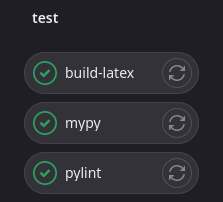
\includegraphics[width=0.5\columnwidth]{./images/gitlab-pipeline.PNG}
		\caption{GitLab Pipeline Web Crawler}
		\label{fig:pipeline}
	\end{center}
\end{figure}

\subsubsection{MongoDB}\label{mongoDB}

MongoDB ist eine dokumentenorientierte NoSQL-Datenbank, die auf flexible
Datenmodellierung und Skalierbarkeit ausgelegt ist. Im Gegensatz zu
relationalen Datenbanken verwendet MongoDB keine Tabellen, sondern
speichert Daten in Dokumenten, die in \gl{collection}s organisiert sind.
Dies ermöglicht eine einfache Handhabung von unstrukturierten Daten
und eine schnelle Abfrage von Informationen. Diese Eigenschaften
ermöglichten uns eine schnelle und flexible Entwicklung des Programmcodes.

MongoDB bietet auch ein umfangreiches Set von Funktionen wie Aggregation,
Indexierung und Volltextsuche.

Ausführlichere Informationen zu MongoDB sind auf der offiziellen Webseite
\footnote{https://www.mongodb.com/} zu finden. Zum Einbinden des Treibers
und der Verwendung mittels Python haben wir öffentlich zugängliche Tutorials
der offiziellen Seite von MongoDB\footnote{https://pymongo.readthedocs.io/en/stable/index.html}
und der Seite GeeksForGeeks \footnote{https://www.geeksforgeeks.org/python-mongodb-tutorial/} verwendet.

\subsubsection{Natural Language Processing (NLP)}

Natural Language Processing (NLP) beschäftigt sich mit der Verarbeitung
von natürlicher Sprache durch Computer und ermöglicht es, diese in eine
für Maschinen verständliche Form zu bringen. Dabei kommen
Algorithmen und Techniken zum Einsatz, die es ermöglichen, Texte zu
verstehen, zu analysieren und zu generieren. Dazu werden häufig Libraries
wie \gl{spacy} (vgl. Abschnitt \ref{spacy}) oder NLTK \footnote{https://www.nltk.org/} verwendet.

\subsubsection{Named Entity Recognition (NER)}

\gl{ner} ist eine \gl{nlp} Technologie und ermöglicht
das automatische Identifizieren von Entitäten mit Namen wie Personen,
Orten, Organisationen und Produkten in Texten. Die in diesem Projekt
geschriebene Software verwendet \gl{ner} von \gl{spacy}

\subsubsection{Part Of Speech (POS) Tagging}

\gl{pos} Tagging ist eine \gl{nlp} Funktionalität, die dazu dient, die Wortarten
(Nomen, Verb, Adjektiv...) aller Wörter in einem Satz zu bestimmen.
Im Allgemeinen werden für \gl{pos} \gl{ml} gestützte Programme verwendet,
um die Zuordnung der Wörter zu den jeweiligen Kategorien zu bestimmen.

\subsubsection{Coreference Resolution}

\gl{cr} ist eine Technik der Sprachanalyse, die darauf abzielt, Pronomen, Artikel und Synonyme im Text
auf ihre Referenz im selben Text zu beziehen. Sie identifiziert das Substantiv, auf das
sich ein Wort bezieht, um eine eindeutige Bedeutung des Satzes
zu ermöglichen. Coreference Resolution ist ein wichtiger Schritt bei der 
automatisierten Textanalyse und ermöglicht es, die Bedeutung von Texten besser zu 
verstehen. In dem Fall dieses Projekts ermöglicht die Zuordnung der Pronomen zu
den Personen eine effizientere Bestimmung des Geschlechts der Person. Da diese
zum Teil Hinweise zum Geschlecht einer Person enthalten (er, sie, sein, ihr...).

\subsubsection{Dependency Parsing}

Dependency Parsing ist eine Technik des \gl{nlp}s, die Beziehungen
zwischen Wörtern in einem Satz untersucht und hierarchisch darstellt.
Dabei wird jeder Satz in eine Baumstruktur umgewandelt, in dem jedes
Wort einen Knoten darstellt und die Beziehungen zwischen den Wörtern durch
Kanten dargestellt werden. Die Beziehungen sind abhängig von der Bedeutung
des Satzes und geben an, welches Wort mit welchem anderen Wort zusammenhängt.

\subsubsection{Spacy}\label{spacy}

\gl{spacy} ist eine Open-Source-Bibliothek für \gl{nlp}, die in Python geschrieben wurde.
Sie bietet Entwickler:innen eine Vielzahl von Funktionen zur Verarbeitung von
Texten, einschliesslich Tokenisierung, \gl{pos}-Tagging, \gl{ner} und
\gl{dependency-parsing}. Spacy wurde für hohe Leistung und Geschwindigkeit entwickelt
und ist auf die Verarbeitung grosser Textmengen ausgelegt. Die Library verfügt über Modelle,
die in mehreren Sprachen verfügbar sind und es ermöglichen, Texte in verschiedenen
Sprachen zu verarbeiten.

In unserem Projekt haben wir das Spacy Modell \enquote{de\_core\_news\_lg}
\footnote{https://spacy.io/models/de/\#de\_core\_news\_lg} verwendet, um die
Funktionen \gl{ner}, \gl{pos}-Tagging und \gl{dependency-parsing} auf deutschsprachige
Texte anzuwenden.